% !TeX root = ../geometry_main.tex
%================================================
%========================================================
\chapter{Differential forms \& integration} \todotag{To be written}
%=========================================================
%===================================================================


\begin{mytheorem}[Indices bookkeeping for differential forms]
The canonical basis for $\Lambda^k(M)$ is written as $dx^{i_1} \wedge \cdots \wedge dx^{i_k}$ with $i_1 < i_2 < \cdots < i_k$.
We will insetad use indices $\sigma_1, \dots, \sigma_k \subseteq \{1, \dots, n\}$ to denote unordered indices.
A $k$-form $\omega \in \Lambda^k (M)$ can be written equivalently as
\begin{align}\label{eq:indices_bookkeeping_differential_forms}
\begin{aligned}
    \omega &= \sum_{i_1 < \cdots < i_k} \omega_{i_1 \dots i_k} dx^{i_1} \wedge \cdots \wedge dx^{i_k}
    \\
    &= \frac{1}{k!} \sum_{\sigma_1, \dots, \sigma_k} \omega_{\sigma_1 \dots \sigma_k} dx^{\sigma_1} \wedge \cdots \wedge dx^{\sigma_k}
    \\
    &= \sum_{\sigma_1, \dots, \sigma_k} \omega_{\sigma_1 \dots \sigma_k}\, dx^{\sigma_1} \otimes \cdots \otimes dx^{\sigma_k},
\end{aligned}
\end{align}
In the first expression we do not sum over repeated indices, which are ordered $i_1 \dots i_k$.
In the second expression we instead sum over the \emph{unordered} indices $\sigma_1, \dots, \sigma_k$, we define $\omega_{\sigma_1 \dots \sigma_k}$ to be totally antisymmetric, and divide by $k!$ to avoid overcounting.
In the third expression we explicitate the wedge product in terms of antisymmetrized tensor product: because $\omega_{\sigma_1 \dots \sigma_k}$ is already totally antisymmetric, and we are still summing over the $\sigma$ indices, the double counting cancel $1/k!$ factor.
\end{mytheorem}


%-----------------------------------------------------
%========================================================
\section{Derivatives on differential forms} \todotag{To be written}
%=========================================================
%-----------------------------------------------------
For differential forms (anti)-derivatives of degree $k\in \mathbb{Z}$ obeys the Leibniz rule in the form
\begin{equation}
    \delta: \Lambda^\bullet (M) \to \Lambda^{\bullet+k} (M), \qquad \delta (\alpha \wedge \beta) = (\delta \alpha) \wedge \beta + (\pm1)^{|\alpha|} \alpha \wedge (\delta \beta).
\end{equation}
Note the sign is well-defined since differential forms are graded-commutative, i.e. $\alpha \wedge \beta = (-1)^{|\alpha||\beta|} \beta \wedge \alpha$.

\begin{mytheorem}[Lie derivative on differential forms]
The Lie derivative is a well-behaved derivative of degree $(0,0)$ on differential forms, defined as the restriction of the usual Lie derivative on tensors.
From the Leibniz rule for tensors and the linearity of the antisymmetrization map, it immediately follows that the Lie derivative also obeys the Leibniz rule wrt the wedge product
\begin{equation}
    \mathcal{L}_X(\alpha \wedge \beta) = (\mathcal{L}_X \alpha) \wedge \beta + \alpha \wedge (\mathcal{L}_X \beta).
\end{equation}
\end{mytheorem}


\begin{mytheorem}[Inner derivative]
The inner derivative is a \emph{anti}derivative of degree $(0,-1)$ on differential forms, defined as the contraction along a vector field $X$
\begin{equation}
    i_X: \Lambda^k (M) \to \Lambda^{k-1} (M)\quad  \mid\quad  i_X \omega := \omega (X, \cdot, \cdots, \cdot) 
\end{equation}
In a basis of $\Lambda^{k-1}(M)$ i.e. for \emph{ordered} indices $i_1< \dots <i_{k-1}$, but summing over \emph{any} value $\sigma\in \{1\dots n\}$, we have
\begin{equation}\label{eq:interior_derivative_basis_expr}
   (i_X \omega) = X^{\sigma}\, \omega_{\sigma i_1 \dots i_{k-1}} \, dx^{i_1} \wedge \cdots \wedge dx^{i_{k-1}}
\end{equation} 
where again $\omega_{\sigma_0 \dots \sigma_k}$ is totally antisymmetric.
Indeed, using the convention \eqref{eq:indices_bookkeeping_differential_forms}, we have
\begin{align}
\begin{aligned}
    i_X(\omega) &= \sum_{\sigma_0 \dots \sigma_{k-1}} \omega_{\sigma_0 \dots \sigma_{k-1}}\, dx^{\sigma_0}\otimes \cdots \otimes dx^{\sigma_{k-1}}\, (X, \cdots)
    \\
    &= \sum_{\sigma_0 \dots \sigma_{k-1}} X^{\sigma_0} \, \omega_{\sigma_0 \sigma_1 \dots \sigma_{k-1}}dx^{\sigma_1}\otimes \cdots \otimes dx^{\sigma_{k-1}}
    \\
    &= \sum_{\sigma_0 \in\{1\dots n\},\,\,i_1 < \cdots < i_{k-1}} X^{\sigma_0} \, \omega_{\sigma_0 i_1 \dots i_{k-1}}\,\,dx^{i_1}\wedge\cdots \wedge dx^{i_{k-1}}.
\end{aligned}
\end{align}
\end{mytheorem}


\begin{mytheorem}[Exterior derivative]
The exterior derivative is an \emph{anti}derivative of degree $(0,1)$ on differential forms, defined as the unique map
\begin{equation}
    d: \Lambda^k (M) \to \Lambda^{k+1} (M)
\end{equation}
that reduces to the usual differential when acting on functions and satisfies $d^2 = 0$.
Under this conditions, one proves the usual formula in a coordinate basis
\begin{equation}\label{eq:exterior_deriv_basis_expr}
    d \Big(\omega_{i_1 \dots i_k} dx^{i_1} \wedge \cdots \wedge dx^{i_k}\Big) = \partial_\mu \omega_{i_1 \dots i_k} \, dx^{\mu} \wedge dx^{i_1} \wedge \cdots \wedge dx^{i_k}.
\end{equation}
\end{mytheorem}


\begin{mytheorem}[Replacing partial with covariant derivatives]
The exterior derivative on a form $\omega=\omega_{i_1 \dots i_k} dx^{i_1} \wedge \cdots \wedge dx^{i_k}$ can equivalently be written in terms of covariant derivatives associated to a torsion-less connection,
\begin{align}
    d\omega &= \partial_\mu \omega_{i_1 \dots i_k} \, dx^{\mu} \wedge dx^{i_1} \wedge \cdots \wedge dx^{i_k}
    \equiv
    \nabla_\mu \omega_{i_1 \dots i_k} \, dx^{\mu} \wedge dx^{i_1} \wedge \cdots \wedge dx^{i_k}.
\end{align}
Indeed both expressions define tensors, the latter by definition of covariant derivative and the former by construction.
Since they coincide in normal coordinates where the Christoffel symbols vanish, they coincide in any coordinate system.
%
\end{mytheorem}

%-----------------------------------------------------
%========================================================
\section{Integration} \todotag{To be written}
%=========================================================
%-----------------------------------------------------
\begin{mytheorem}[Integration of differential forms]
Given an oriented submanifold $S^{(k)} \subseteq M^{(n)}$ of dimension $k$, we can integrate $k$-forms $\omega \in \Lambda^k (M)$ over $S$.
Namely, given a parametrization $\phi: U \subseteq \mathbb{R}^k \to S \subseteq M$, we define
\begin{equation}
    \int_S \omega := \int_U \phi^* (\omega).
\end{equation}
Note that $\phi^* (\omega) \in \Lambda^k (U)$ is a $k$-form on $\mathbb{R}^k$, which can be written as $f(x) dx^1 \wedge \cdots \wedge dx^k$ for some function $f: U \to \mathbb{R}$, and then integrated as usual.
The orientation of $S$ is necessary to have a well-defined integral, since changing the orientation changes the sign of the integral, but orientability of $M$ is not necessary.
\end{mytheorem}

\begin{mytheorem}[Stokes theorem]
This is simply the fundamental theorem of calculus for differential forms.
Namely, for any \emph{oriented} manifold $M^{(n)}$ with boundary $\partial M$ and any differential form $\omega \in \Lambda^{n-1} (M)$, we have
\begin{equation}
    \int_M d\omega = \int_{\partial M} \omega.
\end{equation}
In particular, Stokes theorem formalizes a fundamental relation between the purely algebraic property $d^2 = 0$ and the purely geometric property $\partial ^2 M =0$ i.e. the `boundary of a boundary is empty'.
\end{mytheorem}


%-----------------------------------------------------------------------------
\subsection{Rediscovering familiar operations}
%-----------------------------------------------------------------------------

\begin{mytheorem}[Divergence \& Gauss theorem.]
Given a volume form $\Omega$ and a vector field $X$ on a manifold $M^{(n)}$, define the \textbf{divergence} as the $n$-form
\begin{equation}
    \mathrm{div}_\Omega (X) := \mathcal{L}_X \Omega = d (i_X \Omega) + i_X \graycancel{d\Omega} = d (i_X \Omega).
\end{equation}
Note that this definition is independent of the notion of metric once we are given a volume form $\Omega$.
We can compute the divergence using the expressions \eqref{eq:interior_derivative_basis_expr}-\eqref{eq:exterior_deriv_basis_expr} for $i_x$ and $d$, but it is much easier to use the Leibniz rule for $\mathcal{L}$.
Writing $\Omega = a(x) dx^1 \wedge \cdots \wedge dx^n$ for some nowhere-vanishing function $a$
\begin{align}
    \mathrm{div}_\Omega (X) 
    &= \big(\mathcal{L}_X a\big)\,\,dx^1 \wedge \cdots \wedge dx^n + a(x) \sum_{\mu=1}^n dx^1 \wedge \cdots \wedge \mathcal{L}_X(dx^\mu) \wedge \cdots \wedge dx^n
    \\&= X(a) \, dx^1 \wedge \cdots \wedge dx^n + a(x) \sum_{\mu=1}^n dx^1 \wedge \cdots \wedge dX^{\mu} \wedge \cdots \wedge dx^n
    \\&= \left( X(a) + a(x) \sum_{\mu=1}^n \partial_{\mu} X^{\mu} \right) dx^1 \wedge \cdots \wedge dx^n 
    \\&= \left( \frac{1}{a(x)} \partial_{\mu} \big(a(x) X^{\mu}\big) \right) \, \Omega.
\end{align}
Note that we recover the usual formula for divergence in $\mathbb{R}^n$ when $a(x) = 1$.
\smallskip

More generally, when $\Omega = \sqrt{|g|} dx^1 \wedge \cdots \wedge dx^n$ is the \textbf{metric volume form}, we have
\begin{equation}
    \mathrm{div}_g (X) = \left( \frac{1}{\sqrt{|g|}} \partial_{\mu} \Big(\sqrt{|g|} X^{\mu}\Big) \right) \Omega_g = \left( \nabla_{\mu} X^{\mu} \right) \Omega_g.
\end{equation}
The last equality follows from the definition $\nabla_{\mu}X^\mu= \partial_\mu X^\mu + \Gamma_{\mu \nu}^\mu X^\nu$ and the well-known identity $\Gamma_{\mu \nu}^\mu = \frac{1}{\sqrt{|g|}} \partial_\nu \sqrt{|g|}$ proven in \eqref{eq:metric_christoffel_contraction_identity}.
\smallskip

\textbf{Gauss theorem} is immediately proved using Cartan formula and Stokes theorem.
Let $M$ be an oriented manifold with boundary $\partial M$ and $X$ a vector field.
Then
\begin{equation}
    \int_M \mathrm{div}_\Omega (X) = \int_M \mathcal{L}_X \Omega = \int_M d (i_X \Omega) + i_X \graycancel{d\Omega} = \int_{\partial M} i_X \Omega.
\end{equation}
In the case $\Omega$ is the volume form induced by a metric $g$, we can rewrite the right-hand side and get
\begin{equation}
    \int_M \mathrm{div}_g (X) = \int_{\partial M} i_X \Omega_g = \int_{\partial M} g(X, N)\,\, \tilde{\Omega}_{g|\partial M},
\end{equation}
where $N$ is the outward-pointing unit normal vector field on $\partial M$ and $\tilde{\Omega}_{g|\partial M}$ is the volume form induced by the metric on $\partial M$.

It is indeed immediate to check that $i_X \Omega_g = g(X,N) \tilde{\Omega}_{g|\partial M}$.
By definition, the metric volume form on a metric manifold $(N^{(d)},h)$ is the unique $d$-form such that $\tilde{\Omega}_h (Y_1, \dots, Y_d) = 1$ for any orthonormal positively oriented basis $\{Y_j\}$ at any point $p\in N$.
By the `outward-normal first' convention, if $\{Y_j\}$ is an orthonormal oriented basis of $T_p \partial M$, then $\{N, Y_1, \dots, Y_{n-1}\}$ is an orthonormal oriented basis of $T_p M$.
In turn by definition
{\small
\begin{align}
    i_X&\Omega_g(Y_1, \dots, Y_{n-1}):= \Omega_g (X, Y_1, \dots, Y_{n-1})\\
    &= g(X,N) \underbrace{\Omega_g (N, Y_1, \dots, Y_{n-1})}_{=1} + \sum_j^{n-1} g(X,Y_j) \underbrace{\Omega_g(Y_j, Y_1, \dots)}_{=0} = g(X,N)
    \quad \Rightarrow \quad i_X \Omega_g = g(X,N) \tilde{\Omega}_{g|\partial M}. 
\end{align}
}
A different proof explicitly using coordinates is given below.

In turn, we have the notion of \textbf{integration by parts}.
First note that for any \emph{arbitrary} volume form
\begin{equation}
    df\wedge i_x \Omega = \left(\partial_\mu f \,dx^\mu\right)\wedge \left(X^{\nu_1} \Omega_{\nu_1 \dots \nu_n} dx^{\nu_2} \wedge \cdots \wedge dx^{\nu_n}\right) = \partial_\mu f X^{\mu}\,\, \Omega = df(X) \,\Omega.
\end{equation}
Then we have 
\begin{equation}
    \int_{\partial M} f\,\, i_X \Omega = \int_M d(f\, i_X \Omega) = \int_M df \wedge i_X \Omega + f\, d i_X\Omega = \int_M df(X) \,\Omega + \int_M f\, \mathrm{div}_\Omega (X).
\end{equation}
In case $\Omega = \sqrt{|g|} dx^1 \wedge \cdots \wedge dx^n$ is the metric volume form this reads
\begin{align}
\begin{aligned}
    \int_{M} f\, \underbrace{\nabla_\mu X^{\mu} \, \Omega_g}_{\mathrm{div}_g(X)}
    &= \int_{\partial M} f\,\, i_X\Omega_g\, - \int_M \underbrace{df(X)}_{= X^{\mu} \partial_\mu f} \, \Omega_g
    = \int_{\partial M} f\,\, g(X,N)\, \tilde{\Omega}_{g|\partial M} - \int_M \underbrace{X^{\mu} \partial_\mu f}_{=g(X,\nabla f)}\, \Omega_g,
\end{aligned}
\end{align}
where $\tilde{\Omega}_{g|\partial M}$ is the volume form induced by the metric on $\partial M$ and $N$ is the outward-pointing unit normal vector field on $\partial M$.
\end{mytheorem}
\begin{proof}
We prove the identity $i_X \Omega_g = g(X,N) \tilde{\Omega}_{g|\partial M}$ using coordinates.
Let $\{x^\mu\}_{\mu=0\dots n}$ be coordinates adapted to the boundary i.e. locally $\partial M=\{x^0 = \text{const.}\}$, so that the outward normal can be written $N = \frac{g^{0\mu}}{\sqrt{g^{00}}} \partial_\mu$.
Let $\phi:\partial M \to M$ be any embedding of the boundary into the manifold, so that in the $x^\mu$ coordinates $\phi^0\equiv \text{const.}$.
If $\{y^1\dots y^n\}$ are arbitrary coordinates on $\partial M$, then $\{\partial_{y^a}\phi\}_{a=1\dots n}$ span $T_p \partial M$ and $\{N, \partial_{y^a}\phi\}$ span $T_p M$.
The metric coefficients in the two bases are related by
{\small
\begin{align}
    &\begin{pmatrix}
    \underbrace{g(N,N)}_{=1} & \underbrace{g(N, \tfrac{\partial \phi}{\partial y^a})}_{=0} \\
    \underbrace{g(N, \tfrac{\partial \phi}{\partial y^a})}_{=0} & g(\tfrac{\partial \phi}{\partial y^a}, \tfrac{\partial \phi}{\partial y^b})
    \end{pmatrix}
    = \begin{pmatrix}
    N^0 & \underbrace{\tfrac{\partial \phi^0}{\partial y^a}}_{\equiv 0}
    \\
    N^i & \tfrac{\partial \phi^i}{\partial y^a}
    \end{pmatrix}^T g\Big(\tfrac{\partial}{\partial x^\mu}, \tfrac{\partial}{\partial x^\nu}\Big)
    \begin{pmatrix}
    N^0 &  \underbrace{\tfrac{\partial \phi^0}{\partial y^a}}_{\equiv 0}
    \\
    N^i & \tfrac{\partial \phi^i}{\partial y^a}
    \end{pmatrix}\\[4pt]
    &\quad 
     \Rightarrow\quad \det \big(g(\partial_{y^a} \phi, \partial_{y^b} \phi)\big) = (N^0)^2\, \det\big(\tfrac{\partial \phi^i}{\partial y^a}\big)^2\, \det(g_{\mu \nu}).
\end{align}
}
Pulling back to $\partial M$ the form $i_X \Omega_g$ along $\phi$, using the above relation for determinants and noting that $g(X,N)= g_{\mu\nu}X^\mu N^\nu = X^\mu g_{\mu\nu} \tfrac{g^{0\nu}}{\sqrt{g^{00}}}= \tfrac{X^0}{N^0}$, we have
{\small
\begin{align}
    \phi^*\Big(i_X\Omega_g\Big) &= \phi^*\Big( \sqrt{\det(g_{\mu \nu})}\, \epsilon_{\alpha,\beta_1\dots\beta_n} X^\alpha \frac{1}{n!} dx^{\beta_1} \wedge \cdots \wedge dx^{\beta_n} \Big)\\
    &= \sqrt{\det(g_{\mu \nu})} X^\alpha \underbrace{\epsilon_{\alpha,\beta_1\dots\beta_n}  \frac{1}{n!} d\phi^{\beta_1} \wedge \cdots \wedge d\phi^{\beta_n}}_{=\epsilon_{\alpha 1 \dots n} d\phi^1\wedge \cdots \wedge d\phi^n}\\
    &= \sqrt{\det(g_{\mu \nu})}\, X^0 d\phi^1\wedge \cdots \wedge d\phi^n\\
    &= \sqrt{\det g(\partial_{y^a} \phi, \partial_{y^b} \phi)}\, \frac{X^0}{N^0} \underbrace{\det\big(\partial_{y^a}\phi^i\big)^{-1} d\phi^1\wedge \cdots \wedge d\phi^n}_{=dy^1 \wedge \cdots \wedge dy^n}\\
    &= \sqrt{\det g_{|_{\partial M}}(\tfrac{\partial}{\partial y^a},\tfrac{\partial}{\partial y^a})} g(X,N) \, dy^1 \wedge \cdots \wedge dy^n =: g(X,N)\, \tilde{\Omega}_{g|\partial M}.
\end{align}
}
\end{proof}


\begin{mytheorem}[Curl \& 3D Stokes theorem.]
Given a \emph{Riemannian} manifold $(M,g)$ of dimension $3$ and a vector field $X$, define the 1-from $g(X,\cdot)$, that is lower an index $X_\mu=g_{\mu \nu} X^{\nu}$.
Define the curl as the 2-from obained by taking the exterior derivative
\begin{equation}
    \mathrm{curl} (X) := d (g(X,\cdot)) = d \Big(X_{\mu} \wedge dx^{\mu}\Big).
\end{equation}
Note that in $\mathbb{R}^3$ with the standard Euclidean metric, this definition coincides with the usual notion of curl.
\smallskip

The general Stokes theorem immediately gives the familiar version in $\mathbb{R}^3$:
\begin{equation}
    \int_S \mathrm{curl} (X) =\int_S d (g(X,\cdot)) = \int_{\partial S} g(X,\cdot),
\end{equation}
for any oriented surface $S$ with boundary $\partial S$.
\end{mytheorem}


\begin{mytheorem}[Complex integration \& Gauss-Green Theorem.]
Consider the complex plane as a Riemannian manifold $(\mathbb{R}^2, g)$ with the standard Euclidean metric.
Given a complex homolorphic function $f: \mathbb{C} \to \mathbb{C}$, both the real and imaginary parts \todotag{Finish this}
\end{mytheorem}


%-----------------------------------------------------
%========================================================
\section{Hodge dual \& friends} 
%=========================================================
%-----------------------------------------------------

\begin{mytheorem}[Hodge dual]
%
Given a pseudoriemannian manifold \((M^{(n)}, g)\), write the metric volume form as
\begin{equation}
    \Omega = \sqrt{|g|}dx^1 \wedge \cdots \wedge dx^n 
    = \sqrt{|g|} \epsilon_{\alpha_1 \dots \alpha_n} dx^{\alpha_1} \otimes \cdots \otimes dx^{\alpha_n}
    = \frac{1}{n!} \sqrt{|g|} \epsilon_{\alpha_1 \dots \alpha_n} dx^{\alpha_1} \wedge \cdots \wedge dx^{\alpha_n},
\end{equation}
where the first expression is \emph{not} summed over indices, while the latter two are, and $\epsilon_{\alpha_1 \dots \alpha_n}$ is the Levi-Civita totally antisymmetric \emph{symbol} $\epsilon_{1 2 \dots n} = +1$, not the tensor.

The Hodge dual is the map
\begin{align}
    \star: \Lambda^k (M) &\to \Lambda^{n-k} (M) \quad \mid \quad \theta \mapsto \tfrac{1}{k!}\Omega_g(\theta^{\#}, \cdots),
\end{align}
where \(\theta^{\#}\) is the tensor of rank $(k,0)$ obtained by raising all indices of $\theta$ with the metric.
That is, transform a $k$-form into a $(k,0)$-tensor and then feed it to the first $k$ slots of the volume form to get a $(n-k)$ form and divide by symmetry factors.
The factor $1/k!$ is inserted to avoid overcounting, since both $\theta$ and $\Omega$ are totally antisymmetric in all indices, so that $\star\star = (-1)^{k(n-k)}$ up to signs.
%
Explicitly, with the index convention \eqref{eq:indices_bookkeeping_differential_forms} for {\small $j_1<\cdots<j_k$} ordered and {\small $\mu_1\cdots\mu_k$} arbitrary, the form $\theta$ is
{\small
\begin{align}
    \theta &= \theta_{j_1 \dots j_k} dx^{j_1} \wedge \cdots \wedge dx^{j_k} = \theta_{\mu_1 \dots \mu_k} dx^{\mu_1} \otimes \cdots \otimes dx^{\mu_k}\quad \Rightarrow \quad \theta^{\#} = g^{\mu_1 \alpha_1} \cdots g^{\mu_k \alpha_k} \theta_{\mu_1 \dots \mu_k} \partial_{\alpha_1}\otimes \cdots \otimes \partial_{\alpha_k}.
\end{align}
}
The Hodge dual of the \(k\)-form \(\theta\) is then 
{\small
\begin{align}\label{eq:hodge_dual_first_exp}
    \star \theta &:= \tfrac{1}{k!}\Omega_g(\theta^{\#}, \cdots)
    = \tfrac{1}{k!}\sqrt{|g|}\epsilon_{\beta_1\dots \beta_n} dx^{\beta_1} \otimes \cdots \otimes dx^{\beta_n} \left( g^{\mu_1 \alpha_1} \cdots g^{\mu_k \alpha_k} \theta_{\mu_1 \dots \mu_k} \partial_{\alpha_1}\otimes \partial_{\alpha_k}, \cdots \right)
    \\
    &= \tfrac{1}{k!}\sqrt{|g|}\epsilon_{\alpha_1\dots \alpha_k\beta_{k+1}\dots \beta_n} g^{\mu_1 \alpha_1} \cdots g^{\mu_k \alpha_k} \theta_{\mu_1 \dots \mu_k} dx^{\beta_{k+1}} \otimes \cdots \otimes dx^{\beta_n}
    \\
    &= \frac{1}{k!(n-k)!} \sqrt{|g|}\epsilon_{\alpha_1\dots \alpha_k\beta_{k+1}\dots \beta_n} g^{\mu_1 \alpha_1} \cdots g^{\mu_k \alpha_k} \theta_{\mu_1 \dots \mu_k} dx^{\beta_{k+1}} \wedge \cdots \wedge dx^{\beta_n}\,.
\end{align}}
The factor $1/k!$ is precisely inserted since both $\theta_{\mu_1 \dots \mu_k}$ and $\epsilon_{\alpha_1\dots \alpha_k\beta_{k+1}\dots \beta_n}$ are totally antisymmetric, so that the sum over unordered indices $\mu_\ell$ and $\alpha_\ell$ gives $k!$ equal contributions, and we could equivalently enforce one set of indices is ordered $j_1 < \cdots < j_k$ and avoid the $1/k!$ factor, that is
{\small
\begin{align}
    \star \theta &= \frac{1}{(n-k)!} \sqrt{|g|}\epsilon_{\alpha_1\dots \alpha_k\beta_{k+1}\dots \beta_n} g^{j_1 \alpha_1} \cdots g^{j_k \alpha_k} \theta_{j_1 \dots j_k} dx^{\beta_{k+1}} \wedge \cdots \wedge dx^{\beta_n}\\
    &= \frac{1}{(n-k)!} \sqrt{|g|}\epsilon_{j_1\dots j_k\beta_{k+1}\dots \beta_n} g^{\mu_1 j_1} \cdots g^{\mu_k j_k} \theta_{\mu_1\dots\mu_k} dx^{\beta_{k+1}} \wedge \cdots \wedge dx^{\beta_n}.
\end{align}}
%
\todotag{Check signs etc}
The Hodge dual obeys the following important properties.
\begin{itemize}
    %
    \item \textbf{Idempotent up to a sign.} For a metric {\small \(g=(+1\dots+1,-1\dots-1)\)} of signature {\small \((n-s,s)\)}, and any form \(\alpha\) we have
    \begin{align}
        \star \star \alpha = (-1)^{|\alpha|(n-|\alpha|) + s} \alpha
    \end{align}
    %
    \item \textbf{Symmetry wrt $\wedge$ product.} For any two \(k\)-forms \(\alpha, \beta\) of the same degree
    \begin{equation}
        \alpha \wedge \star \beta = \beta \wedge \star \alpha = \langle \alpha, \beta \rangle_g \, \cdot \Omega_g,\quad \text{where}\quad \langle \alpha, \beta \rangle_g = g^{\mu_1 \nu_1} \cdots g^{\mu_k \nu_k} \alpha_{\mu_1 \dots \mu_k} \beta_{\nu_1 \dots \nu_k}
    \end{equation}
    is the pointwise scalar product induced by the metric \(g\) on $(0,k)$-tensors, times the volume form.
    % 
    \item \textbf{Star of a wedge (degree additivity).}
    For any two form $\alpha\in\Omega^p$ and $\beta\in\Omega^q$
    \begin{align}
        \star(\alpha\wedge\beta)
        =\iota_{\beta^\sharp}(\star\alpha)
        =(-1)^{pq}\,\iota_{\alpha^\sharp}(\star\beta).
    \end{align}
    The inner derivative $i_{\beta^{\#}}$ of a $j$-form with respect to the  $(\ell,0)$-tensor $\beta^\sharp$ means contracting the first $\ell$ slots of the form with the tensor, and gives zero if $\ell>j$. That is when $p+q>n$.
    %
\end{itemize}
\end{mytheorem}
\begin{proof}
We prove the idempotency property. Raising indices of \eqref{eq:hodge_dual_first_exp} we get
{\small
\begin{align}
\big(\star\theta\big)^\#= \tfrac{1}{k!}\sqrt{g}\,\epsilon_{\alpha_1\dots \alpha_k\beta_{k+1}\dots \beta_n} \Big(\prod_{a=1}^k g^{\mu_a \alpha_a}\Big) \theta_{\mu_1 \dots \mu_k} \Big(\prod_{b=k+1}^n g^{\beta_b\nu_b}\Big) \partial_{\nu_{k+1}}\otimes \cdots \otimes \partial_{\nu_n}.
\end{align}}
Apllying the Hodge dual and permuting indices of the second $\epsilon$ symbol we get 
{\small
\begin{align}
\star\star\theta &= \tfrac{1}{(n-k)!}\Omega_g\Big(\big(\star\theta\big)^\#, \cdots\Big)\\
&= \tfrac{1}{k!(n-k)!}\big(\sqrt{|g|}\big)^2\,\epsilon_{\alpha_1\dots \alpha_k\beta_{k+1}\dots \beta_n}\,\theta_{\mu_1 \dots \mu_k} \Big(\prod_{a=1}^k g^{\mu_a \alpha_a}\prod_{b=k+1}^n g^{\beta_b\nu_b}\Big) \epsilon_{\nu_{k+1}\dots \nu_n\gamma_1\dots \gamma_k} dx^{\gamma_1} \otimes \cdots \otimes dx^{\gamma_k}\\
&= \tfrac{(-1)^{k(n-k)}}{k!(n-k)!}\big|\!\det{g_{\mu\nu}}\!\big|\,\epsilon_{\alpha_1\dots \alpha_k\beta_{k+1}\dots \beta_n}\,\theta_{\mu_1 \dots \mu_k} \Big(\prod_{a=1}^k g^{\mu_a \alpha_a}\prod_{b=k+1}^n g^{\beta_b\nu_b}\Big) \epsilon_{\gamma_1\dots \gamma_k\nu_{k+1}\dots \nu_n} dx^{\gamma_1} \otimes \cdots \otimes dx^{\gamma_k}.
\end{align}}
Since both $\theta$ and the two instances of $\epsilon$ are totally antisymmetric, the sum over unordered indices $\alpha_a, \mu_a$ and $\beta_b,\nu_b$ yield $k!$ and $(n-k)!$ equal contributions respectively.
We thus remove the symmetry factor and order indices $\mu_1\dots\mu_k\mapsto i_1<\cdots < i_k$ and $\nu_{k+1}\dots \nu_n\mapsto j_{k+1}<\cdots < j_n$ to get
{\small
\begin{align}
\star\star\theta &= (-1)^{k(n-k)}(-1)^s\det(g_{\mu\nu})\theta_{i_1 \dots i_k} \epsilon_{\alpha_1\dots \alpha_k\beta_{k+1}\dots \beta_n}\Big(\prod_{a=1}^k g^{i_a \alpha_a}\prod_{b=k+1}^n g^{j_b\beta_b}\Big) \epsilon_{\gamma_1\dots \gamma_k j_{k+1}\dots j_n} dx^{\gamma_1} \otimes \cdots \otimes dx^{\gamma_k},
\end{align}}
for the metric signature $s$.
The symbol $\epsilon_{\alpha_1\dots \alpha_k\beta_{k+1}\dots \beta_n}$ yield a generic permutation of $\{1\dots n\}$ so that
{\small
\begin{align}
\epsilon_{\alpha_1\dots \alpha_k\beta_{k+1}\dots \beta_n}\Big(\prod_{a=1}^k g^{i_a \alpha_a}\prod_{b=k+1}^n g^{j_b\beta_b}\Big) = \begin{cases}
    \sum_\sigma\epsilon_{\sigma_1\dots\sigma_n}\prod_{c=1}^n g^{\sigma_c \sigma_c} = \det(g^{\mu\nu})& \text{if } \{i_1\dots i_k\} \cap \{j_{k+1}\dots j_n\} = \emptyset\\[3pt]
    0 & \text{otherwise}.
\end{cases}
\end{align}}
Finally, if $\{i_1\dots i_k\} \cap \{j_{k+1}\dots j_n\} = \emptyset$ then $\epsilon_{\gamma_1\dots \gamma_k j_{k+1}\dots j_n}\neq0$ only if $\{\gamma_1\dots \gamma_k\} = \{i_1\dots i_k\}$.
Since both $i_a$ and $j_b$ are ordered, the sign of $\epsilon_{\gamma_1\dots \gamma_k j_{k+1}\dots j_n}$ can be absorbed into $\theta_{\gamma_1\dots \gamma_k}$ with the usual convention that $\theta$ is antisymmetric in unordered indices, so that we eventually get
{\small
\begin{align}
\star\star\theta &= (-1)^{k(n-k)}(-1)^s\,\cancel{\det(g_{\mu\nu})}\,\cancel{\det(g^{\mu\nu})}\,\theta_{\gamma_1\dots \gamma_k} dx^{\gamma_1} \otimes \cdots \otimes dx^{\gamma_k} = (-1)^{k(n-k)+s} \theta.
\end{align}}
\end{proof}


\begin{mytheorem}[The Hodge scalar product on differential forms.\todotag{Finish this}]
Given two \(k\)-forms \(\alpha, \beta\) on a pseudoriemannian manifold \((M,g)\), the Hodge scalar product is
\begin{equation}
    \langle \alpha, \beta \rangle_{\,\mathrm{Hodge}} := \int_M \alpha \wedge \star \beta
    = \int_M \beta \wedge \star \alpha 
    = \int_M \underbrace{\alpha_{\mu_1 \dots \mu_k}\, \beta_{\nu_1 \dots \nu_k} \,g^{\mu_1\nu_1} \dots g^{\mu_k \nu_k}}_{=\langle \alpha, \beta \rangle_g} \,\,\, \Omega_g\,.
\end{equation}
It is indeed \emph{real} and \emph{symmetric} thanks to the Hodge dual properties, and coincides with the metric contraction of the two forms integrated over the manifold via the volume form.
In particular, when \(\alpha = \beta\)
\begin{equation}
    \langle \alpha, \alpha \rangle_{\mathrm{Hodge}} = \int_M \alpha \wedge \star \alpha = \int_M ||\alpha||^2 \,\Omega,
\end{equation}
where \(||\alpha||^2\) is the pointwise norm of \(\alpha\) induced by the metric \(g\).
Note that the signature of this scalar product on $\Lambda^k(M)$ depends on both the degree \(k\) of the forms and the signature of the metric \(g\).
For example, on the subspace of 1-froms $\Lambda^1 (M)$, the Hodge product has the same signature $(n-s,s)$ as the metric \(g\) itself.
\end{mytheorem}


\begin{mytheorem}[The codifferential. \todotag{Finish}]
%
The codifferential \(\delta\) is defined as the adjoint of the exterior derivative \(d\) with respect to the Hodge scalar product\footnote{Beware that $\delta$ is sometimes defined as \emph{minus} the adjoint of $d$ to make the D'Alambertian $\Box =\delta d+d\delta$ positive definite rather than negative in the Riemannian case. It is just a convention.}
\begin{align}
    \langle \delta \alpha, \beta \rangle_{\mathrm{Hodge}} &:= \langle \alpha, d \beta \rangle_{\mathrm{Hodge}} \quad \Rightarrow \quad \delta := (-1)^{\bullet} \star^{-1}d\,\star = (-1)^{n(\bullet-1)+s+1} \star d \,\star\,\,.
\end{align}
Indeed for any  $k$-form \(\alpha\) and $k\!-\!1$ form \(\beta\)
\begin{align}
    \langle \alpha, d\beta \rangle_{\mathrm{H}} 
    &= \langle d \beta, \alpha \rangle_{\mathrm{H}}
    = \int_M d \beta \wedge \star \alpha
    = \graycancel{\int_M d(\beta \wedge \star \alpha)} - \int_M (-1)^{|\beta|} \beta \wedge d\star \alpha
    \\
    &=
    \underbrace{(-1)^{|\beta|+1+(|\alpha|-1)(n-|\alpha|+1)+s}}_{=(-1)^{n(|\alpha|-1)+s}} \int_M  \beta \wedge (\star\star d\star \alpha)
    \equiv
    (-1)^{n(|\alpha|-1)+s+1} \big\langle\, \star d\,\star \alpha\,, \beta \big\rangle_{\mathrm{H}}.  
\end{align}
In a chart we have\todotag{Check formula}
\begin{align}
    (\delta \alpha)_{\mu_1 \dots \mu_{k-1}} 
    &= - \nabla^{\nu} \alpha_{\nu \mu_1 \dots \mu_{k-1}} 
    = - \frac{1}{\sqrt{|g|}} \partial_{\nu} \Big(\sqrt{|g|} g^{\nu \rho} \alpha_{\rho \mu_1 \dots \mu_{k-1}}\Big).
\end{align}
The codifferential is a linear map of degree \((0,-1)\)
\begin{equation}
    \delta: \Lambda^\bullet (M) \to \Lambda^{\bullet-1} (M),
\end{equation}
but it fails the Leibniz rule i.e. it does not respect the wedge product, so it is not an (anti)-derivative.


\smallskip

\noindent
It obeys the fundamental properties.
\begin{itemize}
    \item \textbf{Nilpotency} \(\delta^2 = 0\), from nilpotency of $d$ and indempotency of $\star$ $\Rightarrow$ homology!
    \item \textbf{Poincaré lemma.} Co-closed implies locally co-exact: \(\delta \alpha = 0 \Rightarrow \alpha = \delta \beta\).
    \item \textbf{Adjointness} \(\langle \delta \alpha, \beta \rangle_{\mathrm{Hodge}} = \langle \alpha, d \beta \rangle_{\mathrm{Hodge}}\).
    \item \textbf{Integration by parts} $\displaystyle \int_M d\alpha \wedge \star \beta = \int_M \alpha \wedge \star \delta \beta \quad $ for any \(k\) and $k\!-\!1$ form \(\alpha,\beta\).

    \item \textbf{Relations with star} {$\quad \displaystyle\star \delta = (-1)^{\bullet} d \star \quad \text{and} \quad \delta \star = (-1)^{\bullet +1} \star d.$}
\end{itemize}

\end{mytheorem}


\begin{mytheorem}[Example: Maxwell equations in terms of differential forms \& Hodge dual]
In any dimension $n$, define the electromagnetic field strength 2-form \(F\) as
\begin{equation}
    F := \frac{1}{2} F_{\mu \nu} dx^{\mu} \wedge dx^{\nu}.
\end{equation}
In $4$-dimension the electric and magnetic fields are encoded in the components of $F$ as
\begin{equation}
    F_{\mu \nu} = \qquad F_{\mu\nu} = \begin{pmatrix}
    0 & -E_1 & -E_2 & -E_3 \\
    E_1 & 0 & B_3 & -B_2 \\
    E_2 & -B_3 & 0 & B_1 \\
    E_3 & B_2 & -B_1 & 0
    \end{pmatrix}.
\end{equation}
%
Given a current $n$-vector $J^\mu$, define the current $1$-form lowering the indices with the metric
\begin{equation}
    J := J_{\mu} dx^{\mu}.
\end{equation}
One also defines the current $(n-1)$--form as its Hodge dual
{\small
\begin{align}
    \star J &:= \Omega_g(J^\mu \partial_\mu,\cdots)= \sqrt{|g|}dx^0\wedge \cdots \wedge dx^{n-1} (J^\mu \partial_\mu,\cdots) 
    = \sqrt{|g|}\,\epsilon_{\alpha_0\dots \alpha_{n-1}} dx^{\alpha_0} \otimes \cdots \otimes dx^{\alpha_{n-1}} (J^\mu \partial_\mu,\cdots)
    \\
    &=  \sqrt{|g|}\,\epsilon_{\alpha_0\dots \alpha_{n-1}} J^{\alpha_0}\, dx^{\alpha_1} \otimes \cdots \otimes dx^{\alpha_{n-1}} 
    = \sqrt{|g|}\,\frac{1}{(n-1)!}\epsilon_{\alpha_0\dots \alpha_{n-1}} J^{\alpha_0}\, dx^{\alpha_1} \wedge \cdots \wedge dx^{\alpha_{n-1}}.
\end{align}
}
%
The Maxwell equations read
\begin{equation}
    dF = 0, \qquad \delta F = J \quad \text{or equivalently} \quad d \star F = \star J.
\end{equation}
The first equation encodes the homogeneous Maxwell equations (Faraday law \& no magnetic monopoles), while the second encodes the inhomogeneous ones (Gauss law \& Ampere-Maxwell law).
The first equation \(dF=0\) implies the 2-form is closed and thus locally exact, i.e. there exists a 1-form $A$ identified with the electromagnetic potential such that
\begin{equation}
    F = dA,\qquad A = A_{\mu} dx^{\mu}.
\end{equation}
Moreover, it automatically implies invariance under gauge transformations $A_\mu\mapsto A_\mu + \partial_\mu a$.
\end{mytheorem}




\begin{mytheorem}[Laplace-de Rham-Hodge-D'Alambert operator\todotag{Finish}]
%
The Hodge--de Rham operator \(\Box\) is defined on all, possibly fiber valued, differential forms as
\begin{equation}
    \Box: \Lambda^\bullet(M) \otimes E_F \to \Lambda^\bullet(M) \otimes E_F, \qquad \Box := d \delta + \delta d \equiv (d + \delta)^2.
\end{equation}
It preserves the degree of forms, but it does \emph{not} satisfy the Leibniz rule in any easy sense.
\smallskip

It satisfies the following properties.
\begin{itemize}
    \item \textbf{Commutations.} $d \,\Box = \Box\, d,\quad \delta\, \Box = \Box\, \delta,\quad \star\, \Box = \Box\, \star$.
    \item \textbf{Self-adjoint wrt Hodge product.} \(\langle \Box \alpha, \beta \rangle_{\mathrm{Hodge}} = \langle \alpha, \Box \beta \rangle_{\mathrm{Hodge}}\).
    In the Riemannian case the Hodge product is positive definite, and $\Box$ is thus diagonalizable by the spectral theorem.
    It has nonpositive spectrum $\text{Spec}(\Box)\subseteq (-\infty,0]$ (cf. below).
\end{itemize}
\smallskip

Depending on the signature of the metric \(g\), it generalizes either the Laplacian (Riemannian case), the D'Alambertian (Lorentzian case) or anything in between (general pseudoriemannian case). 
In the Riemannian case it is an elliptic operator (positive semidefinite), while in the Lorentzian case it is hyperbolic.
This is easily seen in flat Euclidean or Minkowski space, passing to Fourier space
\begin{equation}
    p_E^2 = p_1^2 + p_2^2 + p_3^2 + \cdots \geq 0,\quad p_M^2 = p_0^2 - p_1^2 - p_2^2 - \cdots.
\end{equation}
\smallskip

In\todotag{Check formula} a chart, it acts on a $k$-form $\alpha$ as
\begin{align}
    (\Box \alpha)_{\mu_1 \dots \mu_k} 
    =& - \nabla^{\nu} \nabla_{\nu} \alpha_{\mu_1 \dots \mu_k} + \sum_{i=1}^k (-1)^i R^{\rho}_{\ \mu_i} \alpha_{\mu_1 \dots \mu_{i-1} \rho \mu_{i+1} \dots \mu_k} 
    \\
    &  - 2 \sum_{1\leq i < j \leq k} (-1)^{i+j} R^{\rho}_{\,\mu_i \mu_j}{}^{\sigma} \alpha_{\mu_1 \dots \mu_{i-1} \rho \mu_{i+1} \dots \mu_{j-1} \sigma \mu_{j+1} \dots \mu_k},
\end{align}

In particular, on 0-forms i.e. functions it reduces to the usual Laplace-D'Alambert operator
\begin{equation}
    \Box f =  \nabla^{\nu} \nabla_{\nu} f.
\end{equation}
In fact, the Hodge operator could also  be defined as the \textbf{unique operator of degree $0$ on differential forms that reduces to the usual Laplacian/D'Alambert operator on functions and commutes with both \(d\) and \(\delta\).}
\medskip

The Hodge operator $\Box$ can also be understood as the \textbf{square of the Dirac operator} acting on differential forms, defined as
\begin{equation}
    \slashed{D} := d + \delta.
\end{equation}
Indeed, from nilpotency of $\delta$ and $d$ we have $\slashed{D}^2 = (d + \delta)^2 = d^2 + d \delta + \delta d + \delta^2 = d \delta + \delta d = \Box$.

Finally, its action on 0-forms can be understood as the operator yielding the Euler-Lagrange equations for the action of a free scalar field \(\phi\).
Indeed we have 
\begin{equation}
    S[\phi] =  \int_M\!\! \mathrm{d}^n x\, \sqrt{|g|}\,\tfrac{1}{2} \partial_\mu \phi \partial^\mu \phi\
    = \int_M \tfrac{1}{2}  ||d\phi||^2 \Omega_g = \int_M \tfrac{1}{2} d\phi \wedge \star d\phi 
    = \tfrac{1}{2}\langle d\phi, d\phi \rangle_{\mathrm{Hodge}}.
\end{equation}
Varying with respect to \(\phi\mapsto \phi +\varepsilon\), one finds
\begin{equation}
    \delta S[\phi] = \int_M d \varepsilon \wedge \star d\phi = \int_M \graycancel{d\left(\varepsilon \star d\phi\right)} - \varepsilon\,\, d \star d\phi \quad \Rightarrow \quad d \star d\,\,\phi  = 0.
\end{equation}
Equivalently, more abstractly,
\begin{equation}
    \delta S[\phi] = \delta \left(\tfrac{1}{2}\langle d\phi, d\phi \rangle_{\mathrm{Hodge}}\right)
    = \langle d \phi, d \varepsilon \rangle_{\mathrm{Hodge}}
    = \langle \delta d \phi, \varepsilon \rangle_{\mathrm{Hodge}} \quad \Rightarrow \quad \delta\, d\, \phi = 0.
\end{equation}
Since $\delta \simeq \star d\,\star$ and $\delta \phi=0$ for 0-forms, both expressions ultimately gives equation of motion  $\Box\, \phi = 0$.
%
\end{mytheorem}


%-----------------------------------------------------
%========================================================
\section{Spectral geometry} 
%=========================================================
%-----------------------------------------------------

\begin{mytheorem}[Introduction: can you hear the shape of a drum?]
%
Can we detect and describe (pseudo-)Riemannian structures \(\mathcal{E}\) directly, without reference to a particular metric \(g\)?
Possibly yes, using \textbf{spectral geometry}.
The idea is that the vibration spectrum \(\{\lambda_n\}\) of a manifold (the eigenvalues of a Laplace-type operator) depends only on \(\mathcal{E}\) and not on the choice of coordinates.
The classical question of spectral geometry, posed by Hermann Weyl in 1911, is:
%
\begin{center}
\emph{Does the spectrum \(\{\lambda_n\}\) encode all information about the shape, i.e. the structure \(\mathcal{E}\)?}
\end{center}
%
The expectation is that the spectra \(\mathrm{spec}(\Delta_p)\) of the laplacian on fiber valued p-forms for different $p$ and fibers contain different information about $M$, possibly enough to reconstruct its shape completely.
%
\end{mytheorem}


\vspace{-0.3mm}
\begin{wrapfigure}[9]{r}{0.34\textwidth}
  \centering
  \vspace{-\intextsep}
  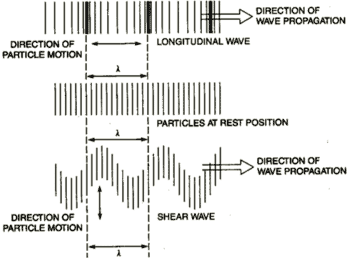
\includegraphics[width=\linewidth]{images/seismic_wave.png}
  %\caption{Shear vs. pressure seismic wave}
  \label{fig:seismic_waves}
\end{wrapfigure}

\noindent
For example, it is known that scalar (a.k.a. pressure, longitudinal) and vector (ak.a. shear, transverse) seismic waves travel and reflect off materials differently, e.g. shear waves propagate slower and do not travel through liquids since liquids do not support shear stresses by definition. Their spectra thus contain different information about the Earth's interior structure. This is indeed how seismologists study the Earth's structure and discovered, for example, that its core is liquid in the outer part and solid in the inner part.
\bigskip


\begin{mytheorem}[Types of waves on \(M\)]
%
On a given manifold we can consider fiber valued p-forms \(w(t)\) with time evolution governed by various differential equations.
%
\begin{enumerate}
\item \textbf{Schrödinger equation }
\(
 i\hbar\,\partial_t w(x,t)
 \;=\; -\frac{\hbar^2}{2m}\,\Delta_p\,w(x,t).
\)
\item \textbf{Heat equation }
\(
 \partial_t w(x,t)
 \;=\; \,\Delta_p\,w(x,t).
\)
\item \textbf{Klein-Gordon/wave equation}
\(
 \,\partial_t^2 w(x,t)
 \;=\; \beta^2\,\Delta_p\,w(x,t),\,
\)
where \(\beta\) is the propagation speed of the given type of wave, e.g. the speed of sound $\beta=c_s$ for pressure waves or the speed of shear waves $ \beta=c_{sh}$.
%
\end{enumerate}
%
Suppose we find an eigenform \(\tilde{\omega}(x)\) of \(\Delta_p\) with eigenvalue \(\lambda\):
\[
 \Delta_p\,\tilde{\omega}(x) \;=\; \lambda\,\tilde{\omega}(x).
\]
Since \(\Delta_p\) is self-adjoint wrt the Hodge inner product \((w,v)=\int_M w\wedge *v\), such eigenforms exist and form an orthonormal basis if $M$ is Riemannian, compact and without boundary (for simplicity).
%
Each evolution equations above is then solved by separation of variables as 
\begin{align*}
 \text{Schrödinger:}&\quad
 w(x,t) \;=\; e^{\tfrac{i\hbar\lambda}{2m}\,t}\,\tilde{\omega}(x),\\[0.3em]
 \text{Heat:}&\quad
 w(x,t) \;=\; e^{-\,2\lambda\,t}\,\tilde{\omega}(x),\\[0.3em]
 \text{Klein–Gordon:}&\quad
 w(x,t) \;=\; e^{i\beta\lambda\,t}\,\tilde{\omega}(x).
\end{align*}
%
It follows that the spectrum \(\mathrm{spec}(\Delta_p)\) is the \emph{overtone spectrum} of p-form type waves on the manifold \(M\).
%
\end{mytheorem}


\begin{mytheorem}[Practical mathematical aspects of spectral geometry]
%
Several practical aspects must be considered regarding the rigorous mathematical formulation of spectral geometry.
%
\begin{itemize}
\item \textbf{(Non)-compact riemannian manifolds} (theorem).
If \((M,g)\) is a compact Riemannian manifold without boundary (it has then finite volume), for each degree $p$ the spectrum \(\mathrm{spec}(\Delta_p)\) of the Laplace-de Rham operator acting on $T^\star_\bullet M$-valued $p$-forms is discrete, with finite degeneracies and without accumulation points.

On the other hand, if the manifold \(M\) has infinite volume (non-compact) then the spectrum of \(\Delta\) must develop a continuous part\footnote{Besides a possible still discrete point-spectrum.}, and we cannot hope to recover information from it since it is the same for all such manifolds, i.e. `all infinite volume drums sound the same'.

\textbf{In practice} one models an arbitrarily large part of the universe by a compact Riemannian manifold \((M,g)\).  This allows us to describe, for example, 3-dimensional space at a fixed time.
%
\item \textbf{Pseudo-Riemannian manifolds}(open problem).
The spectral geometry of \emph{pseudo}-Riemannian manifolds is still very little developed.
The main difficulty is that the Hodge inner product has indefinite signature, so that Laplace-type operators on such manifolds are typically not elliptic and the spectral theorem does not apply.

\textbf{In practice} one typically models spacetime as a compact Riemannian manifold \((M,g)\) after Wick rotation and then tries to recover the Lorentzian structure by analytic continuation.
%
\item \textbf{Boundaries.} The spectral geometry of manifolds is indeed studied.
One needs to impose suitable boundary conditions on the eigenforms of \(\Delta_p\) at \(\partial M\), for example Dirichlet or Neumann conditions.

\textbf{In practice} one typically models space(time) as a compact Riemannian manifold without boundary, or with boundary conditions that effectively make the boundary invisible to the waves considered like periodic BCs.
%
\end{itemize}

\end{mytheorem}

\begin{mytheorem}[Can you hear the shape of a drum? In general no, but often yes.]
%
In general, even in the simplest case of compact Riemannian manifolds without boundary, the spectra of $\Delta$ on \textbf{standard} $\R$\textbf{valued} $p$-forms do \textbf{not contain enough information to uniquely identify the geometric structure}.
Indeed we shall see below that there is relatively little independent information contained in the spectra of $p$-forms because of the many symmetries of $\Delta$ relating the spectra for different $p$.
%
There are indeed examples of pairs \((M,g)\) and \((M',g')\) isospectral for \(\Delta\) on all degrees \(p\), but not isometric.
Nevertheless, all known \textbf{counterexamples have limited physical significance}.
They involve manifolds that are locally, but not globally, isometric (e.g.  one is a $k$-fold covering of the other); manifolds that are $\Delta_p$ isospectral only for some $p$; or manifolds occurring in discrete copies (e.g. mirror images).
%

The situation is different if one considers the spectra of Laplacians acting on more general tensor fields.
For example, rank 2 \textbf{tensor fields} (in particular, metric perturbations) \textbf{contain new information} about the Riemannian structure wrt the sole $p$-forms.
Indeed, a rank-2 tensor can be decomposed into scalar, vector and tensor parts, each with its own spectrum.
While the spectra of scalar and vector parts are related to those of 0- and 1-forms, the tensor part contains genuinely new information not present in the spectra of any $\R$-valued $p$-form.
%
\end{mytheorem}



\begin{mytheorem}[Hodge decomposition: exact, closed and harmonic forms \& spectra of $\Delta$]
%
For simplicity we consider a compact Riemannian manifold $(M,g)$ without boundary or with suitable boundary conditions like DBc or PBc.
\emph{Partial} extensions to pseudo-riemannian manifolds or noncompact ones are possible.

The spaces of differential p-forms admit the \textbf{Hodge decomposition} into subspaces orthogonal wrt the Hodge inner product
\begin{align}
    \Lambda_p \;=\;d\Lambda_{p-1}\;\oplus\;\delta\Lambda_{p+1}\;\oplus\;\Lambda_p^0.
\end{align}
The decomposition holds for arbitrary fiber-valued form since the operators \(d\), \(\delta\) and \(\Delta\) act only on the base manifold, so that 
 \begin{equation}
    \Lambda_p \otimes E_F = \left(d\Lambda_{p-1}\;\oplus\;\delta\Lambda_{p+1}\;\oplus\;\Lambda_p^0\right)\otimes E_F = \left(d\Lambda_{p-1}\otimes E_F\right)\;\oplus\;\left(\delta\Lambda_{p+1}\otimes E_F\right)\;\oplus\;\left(\Lambda_p^0\otimes E_F\right).
\end{equation}
Each subspace is invariant under the action of the Laplace-de Rham operator \(\Delta_p\) because $\Lambda_p^0:=\ker(\Delta_p)$ and the commutation relations \([\Delta,d]=0\) and \([\Delta,\delta]=0\) and $\Lambda_p^0:=\ker(\Delta_p)$.
In particular $\Delta_p$ is invertible on the subspaces of exact and co-exact forms.
Any eigenform of $\Delta$ lies entirely in one of these subspaces and its spectrum decomposes into
\begin{equation}
    \mathrm{spec}(\Delta_p) \;=\; \Big(\,\mathrm{spec}(\Delta_p|_{d\Lambda_{p-1}}) \;\cup\; \mathrm{spec}(\Delta_p|_{\delta\Lambda_{p+1}})\,\Big) \sqcup\; \underbrace{\mathrm{spec}(\Delta_p|_{\Lambda_p^0})}_{\equiv\{0\}}.
\end{equation}
The decomposition is \textbf{irredubile} i.e. there are no further invariant subspaces of \(\Delta_p\).
\end{mytheorem}
\begin{proof}
\todotag{Insert}
\end{proof}

\begin{mytheorem}[Hodge decomposition \& de Rham cohomology]
Each deRham cohomology class contains exactly one harmonic representative, because of the following.
\begin{itemize}
    \item Each harmonic form is closed and co-closed, but neither exact nor co-exact
    \begin{align}
        \Delta \omega = 0 \quad \Longrightarrow \quad d\omega = 0, \quad \delta \omega = 0.
    \end{align}
    \item Every exact (resp. co-exact) form is \emph{not} co-closed (resp. closed)
    \begin{align}
        \alpha = d\beta\,\Rightarrow\, \delta \alpha \neq 0, \qquad \eta = \delta \theta\,\Rightarrow\, d\eta \neq 0.
    \end{align}
\end{itemize} 
The vector space of harmonic p-forms is thus linearly isomorphic to the p-th deRham cohomology group of the manifold
\begin{align}
    \Lambda_p^0 \cong H^p_{dR}(M) := \frac{\ker(d:\Lambda_p\to\Lambda_{p+1})}{\mathrm{im}(d:\Lambda_{p-1}\to\Lambda_p)}\,,\qquad B_p=\dim(H^p_{dR}(M)) = \dim(\Lambda_p^0).
\end{align}
The space $\Lambda_p^0$ is thus a topological invariant of the manifold, independent of the metric \(g\).
This is non-trivial: even though $d$ depends only on the differentiable structure of $M$, the codifferential $\delta$ and hence the Laplacian $\Delta$ does depend on the metric $g$.
\end{mytheorem}
\begin{proof}
\todotag{Insert}
\end{proof}

\begin{mytheorem}[Symmetries of $\Delta$ spectra]
%
The above `(co-)exatcness vs (co-)closedness' properties and the commutations relations $[\Delta,*]=[\Delta,d]=[\Delta,\delta]=0$ of the Laplace operator imply the following isomorphisms and symmetries of $\Delta$ spectra.
\begin{itemize}
    \item \textbf{Hodge duality.} The Hodge map
    \begin{align}
        \star:\underbrace{d\Lambda_{p-1}\oplus \delta\Lambda_{p+1} \oplus \Lambda_p^0}_{\Lambda_p} \longrightarrow \underbrace{d\Lambda_{n-p-1}\oplus \delta\Lambda_{n-p+1} \oplus \Lambda_{n-p}^0}_{\Lambda_{n-p}}
    \end{align}
    is an isomorphism interchaning the decomposition and preserving the spectra of $\Delta$ as 
    \begin{align}
        &\star: d\Lambda_{p-1} \;\longrightarrow\; \delta\Lambda_{n-p+1},\quad \mathrm{spec}(\Delta_{p}|_{d\Lambda_{p-1}}) = \mathrm{spec}(\Delta_{n-p}|_{\delta\Lambda_{n-p+1}}),\\[6pt]
        &\star: \delta\Lambda_{p+1} \;\longrightarrow\; d\Lambda_{n-p-1},\quad \mathrm{spec}(\Delta_{p}|_{\delta\Lambda_{p+1}}) = \mathrm{spec}(\Delta_{n-p}|_{d\Lambda_{n-p-1}}),\\[6pt]
        &\star: \Lambda_p^0 \;\longrightarrow\; \Lambda_{n-p}^0, \qquad \qquad\mathrm{spec}(\Delta_p|_{\Lambda_p^0}) = \mathrm{spec}(\Delta_{n-p}|_{\Lambda_{n-p}^0})\equiv \{0\}.
    \end{align}
    %
    \item \textbf{(Co-)Exact duality.} The following maps are isomorphisms, respect spectra of $\Delta$ 
    \begin{align}
        &d: \delta\Lambda_{p+1} \;\longrightarrow\; d\Lambda_{p},\quad
        \delta: d\Lambda_{p} \;\longrightarrow\; \delta\Lambda_{p+1}, \quad \mathrm{spec}(\Delta_{p+1}|_{d\Lambda_{p}}) = \mathrm{spec}(\Delta_p|_{\delta\Lambda_{p+1}})\\[7pt]
        &\delta\circ d_{|\delta\Lambda_{p+1}} = \Delta_{p|\delta\Lambda_{p+1}},\qquad d\circ \delta_{|d\Lambda_p} = \Delta_{p+1|d\Lambda_p},
    \end{align}
    and the compositions are the restrictions of $\Delta$ to the respective subspaces. 
\end{itemize}
%
This is suggestively shown in the following diagram, where equal colors indicate isomorphic subspaces with identical spectra of $\Delta$,

\begin{samepage}
\begin{align}
  \begin{array}{l}
    {\vdots}\\[0pt]
    \Lambda_{p-1} = {\color{lightblue}d\Lambda_{p-2}}\;\oplus\;{\tikzmarknode{delp}{\color{blue}\delta\Lambda_p}}\;\oplus\;{\color{forestgreen}\Lambda_{p-1}^0}\\[12pt]
    \Lambda_p     = {\tikzmarknode{dp}{\color{blue}d\Lambda_{p-1}}}\;\oplus\;{\tikzmarknode{delp1}{\color{violet}\delta\Lambda_{p+1}}}\;\oplus\;{\tikzmarknode{hp}{\color{yellow}\Lambda_p^0}}\\[8pt]
    \Lambda_{p+1} = {\color{violet}d\Lambda_p}\;\oplus\;{\color{red}\delta\Lambda_{p+2}}\;\oplus\;\Lambda_{p+1}^0\\[0pt]
    {\vdots} \\[0pt]
    \Lambda_{n-p} = {\tikzmarknode{dnp}{\color{violet}d\Lambda_{n-p-1}}}\;\oplus\;{\tikzmarknode{delnp}{\color{blue}\delta\Lambda_{n-p+1}}}\;\oplus\;{\tikzmarknode{hnp}{\color{yellow}\Lambda_{n-p}^0}}\\[6pt]
    \Lambda_{n-p+1} = {\color{blue}d\Lambda_{n-p}}\;\oplus\;{\color{lightblue}\delta\Lambda_{n-p+2}}\;\oplus\;{\color{forestgreen}\Lambda_{n-p+1}^0}\\[0pt]
    {\vdots}
  \end{array}.
\end{align}
%
\begin{tikzpicture}[remember picture,overlay,>=Stealth,shorten >=2pt,shorten <=2pt]
  %\draw[blue,<->] (delp.south) to[bend left=15] node[left=2pt] {\scriptsize $d\!-\!\delta$} (dp.north);
  %\draw[blue,<->] (delp.south) to[bend left=13]node[left=2pt,yshift=4pt] {\scriptsize $d$ - $\delta$}(dp.north);
  \draw[blue,<->] (delp.south) to[bend left=4] node[pos=0.0,left=2pt,yshift=-8pt] {\scriptsize $\delta$} node[pos=0.7,left=2pt,yshift=3pt] {\scriptsize $d$}(dp.north);
  %\draw[yellow,<->]      (hp.south east) -- node[right=2pt] {$\star$} (hnp.north east);
  %\draw[yellow,<->] (hp.south east) to[bend left=15] node[right=2pt] {$\star$} (hnp.north east);
  \draw[yellow,<->] (hp.south east) to[bend left=15] node[right=2pt] {$\star$} ($(hnp.north east)+(-1.6em,0)$);
  %\draw[violet,<->]      (delp1.south east) to[bend left=15] node[right=2pt] {$\star$} (dnp.north east);
  %\draw[blue,<->]        (dp.south east) to[bend left=15] node[right=2pt] {$\star$} (delnp.north east);
  \draw[violet,<->] (delp1.south west) to[bend right=22] node[near end,right=-1pt,yshift=-2pt] {$\star$} ($(dnp.north east)+(-2.5em,0)$);
\draw[blue,<->]   ($(dp.south east)+(-1.9em,0)$)    to[bend left=19] node[near end,right=2pt,yshift=-3pt] {$\star$} ($(delnp.north west)+(0,0)$);
\end{tikzpicture}
\end{samepage}

\noindent
This pattern reveals there is relatively little independent information contained in the spectra of $p$-forms because of the many symmetries of $\Delta$.
%
For example, when \(\dim(M)=3\) 
\begin{align}
\begin{aligned}
  \Lambda_0 \;=\; 0\;\;&\oplus\;{\color{blue}\delta\Lambda_1}\;\oplus\;{\color{forestgreen}\Lambda_0^0}\\
  \Lambda_1 \;=\; {\color{blue}d\Lambda_0}\;&\oplus\;{\color{red}\delta\Lambda_2}\;\oplus\;{\color{green}\Lambda_1^0}\\
  \Lambda_2 \;=\; {\color{red}d\Lambda_1}\;&\oplus\;{\color{blue}\delta\Lambda_3}\;\oplus\;{\color{green}\Lambda_2^0}\\
  \Lambda_3 \;=\; {\color{blue}d\Lambda_2}\;&\oplus\; 0\; \oplus\;{\color{forestgreen}\Lambda_3^0}\,,\\
  .
\end{aligned}
\qquad \text{and}\qquad
\begin{aligned}
  \Lambda_0 \;=\; 0\;\;&\oplus\;{\color{blue}\delta\Lambda_1}\;\oplus\;{\color{forestgreen}\Lambda_0^0}\\
  \Lambda_1 \;=\; {\color{blue}d\Lambda_0}\;&\oplus\;{\color{red}\delta\Lambda_2}\;\oplus\;{\color{green}\Lambda_1^0}\\
  \Lambda_2 \;=\; {\color{red}d\Lambda_1}\;&\oplus\;{\color{red}\delta\Lambda_3}\;\oplus\;{\color{yellow}\Lambda_2^0}\\
  \Lambda_3 \;=\; {\color{red}d\Lambda_2}\;&\oplus\;{\color{blue}\delta\Lambda_4}\;\oplus\;{\color{green}\Lambda_3^0}\\
  \Lambda_4 \;=\; {\color{blue}d\Lambda_3}\;&\oplus\; 0\; \oplus\;{\color{forestgreen}\Lambda_4^0}\,.
\end{aligned}
\end{align}
%
In 3D all the information is contained in the spectra of 0-forms and 1-forms, that is scalar and vector waves.
The same is essentially true in 4D, since harmonic forms are homotopy invariants independent of the metric.
All the information about the curvature of $(M,g)$ is contained in the spectra of $\Lambda_0$ and $\Lambda_1$, while the genuinely new piece of information $\Lambda_2^0$ is only topological and insensitive to the metric $g$.
%
\end{mytheorem}
\begin{proof}
\todotag{Insert}
\end{proof}


\begin{mytheorem}[Perturbative spectral geometry \& Lie exponentiation of infinitesimal changes.]
%    
Geometry is highly nonlinear.
In full generality it is impossible to predict how a finite modification to the shape of a manifold (e.g. growing a bump) will change its spectra.
A possible approach is thus to consider infinitesimal perturbations to a known pseudo-riemannian structure $(M,g)$ and study the corresponding infinitesimal changes in the spectra of its Laplace-type operators.
The infinitesimal changes can then be iterated to reconstuct the full shape of the manifold and corresponding spectra.
This is analogous to the way Lie groups are constructed by exponentiating their Lie algebras. 


Assume both the manifold and its spectra are given: a compact Riemannian manifold \((M,g)\) without boundary and the spectra \(\{\lambda_n^{(p)}\}_n\) of Laplacian operators  \(\Delta\) on $p$-forms and more genrally on tensor fields.
%
In particular, it is possible to define an elliptic self-adjoint Laplacian acting on $T_2(M)$ and find a corresponding orthonormal basis \(\{b_n(x)\}\) with eigenvalues \(\{\lambda_n^{(p)}\}\) satisfying
\begin{equation}
 \Delta\, b_n(x) \;=\; \lambda_n\, b_n(x).
\end{equation}

Now consider an infinitesimal (linear) perturbation to the shape $(M,g)$ and the corresponding infinitesimal (linear) change in  spectra, where $\bullet$ denote suitable tensor types,
\begin{equation}
    g\mapsto g+h\qquad \Rightarrow\qquad \{\lambda_n^{\bullet}\}\,\mapsto\,
 \{\lambda_n^{\bullet}+\mu_n^{\bullet}\}.
\end{equation}
%
The metric perturbation \(h\in T_2(M)\) can be expanded in the above basis as
\begin{equation}
 h \;=\; \sum_{n=1}^\infty h_n\, b_n(x).
\end{equation}
Schematically one can think of adding a bump described by the coefficients \(\{h_n\}_{n=1}^\infty\) to the metric \(g\) and correspondingly shifting the spectra by \(\{\mu_n^{(\bullet)}\}_{n=1}^\infty\).
% 
Concretely, we thus obtain a \emph{linear map}
\begin{equation}
    S\colon \{h_n\}\;\longrightarrow\;\{\mu_n^\bullet\}\quad \mid \quad h_n \mapsto \mu_n^\bullet = S_{mn}\,h_m.
\end{equation}
Sine the manifold is compact, the indices are indeed countable discrete, so that $S$ is an infinite square matrix.
If we further introduce some UV regularization, allowing only eigenvectors and eigenvalues up to some cut-off scale, then we have an (equal) finite number $N$ of parameters \(\{h_n\}_{n=1}^N\) and spectral shifts \(\{\mu_n^{(m)}\}_{n=1}^N\), and $S$ is a finite \(N\times N\) square matrix.
If \(\det S\neq 0\), as it is the case for \emph{general} matrices, then \(S\) is invertible and one can recover \(h\) from the spectral shift.
That is, we can infer the infinitesimal change in the shape from the infinitesimal change in the sound of the (originally known) drum.
One should then iterate these infinitesimal perturbations.

\noindent
\textbf{Further remarks.}
\begin{itemize}
\item Not every perturbation \(h\) actually changes the shape.  If \(h=\mathcal{L}_X g\) for some vector field \(X\) then \(g\mapsto g+h\) is merely the infinitesimal change of chart belonging to the flow generated by \(X\).
\item Symmetric covariant 2-tensors such as \(h\) admit a canonical decomposition similar to the Hodge decomposition.  Accordingly, the Laplacian \(\Delta\) has three distinct spectra on the space \(T_2(M)\) of such tensors.
\end{itemize}

\noindent
\textbf{References.}
This is the subject of ongoing research by Achim Kempf at PI and others.
For more details see, for example, Kempf's talk at the Perimeter Institute: \url{http://pirsa.org/15090062}.
The idea of infinitesimal spectral geometry arises from his paper on how spacetime could be simultaneously continuous and discrete, in the same way that information can.

\end{mytheorem}



%-----------------------------------------------------
%========================================================
\section{Closed vs exact forms \& de Rham cohomology} \todotag{To be written}
%=========================================================
%-----------------------------------------------------

\begin{mytheorem}[Closed \& exact forms]
A differential form \(\omega \in \Lambda^k (M)\) is called \textbf{closed} if \(d\omega = 0\).
It is called \textbf{exact} if there exists a \((k-1)\)-form \(\alpha\) such that \(\omega = d\alpha\).
Because \(d^2 = 0\), every exact form is closed.
The converse is not true in general, as we will see when discussing de Rham cohomology.
\end{mytheorem}


\begin{theorem}[Poincaré lemma]
Let \(M\) be a smooth manifold and let \(U \subseteq M\) be a contractible open subset.
Then, every closed differential form \(\omega \in \Lambda^k (U)\) is exact, i.e. there exists a \((k-1)\)-form \(\alpha\) such that \(\omega = d\alpha\).
This theorem has extensions to more general \emph{homotopically trivial} subsets.
\end{theorem}

